\documentclass[border=10pt]{standalone}
\usepackage{tikz}
\usetikzlibrary{calc}
\usetikzlibrary{backgrounds}
\definecolor{bg}{HTML}{171D2B}
\definecolor{aksen}{HTML}{F7B538}
\definecolor{aksen2}{HTML}{7DD3FC}
\definecolor{putih}{HTML}{FFFFFF}
\definecolor{cermin}{HTML}{94A3B8}

\begin{document}
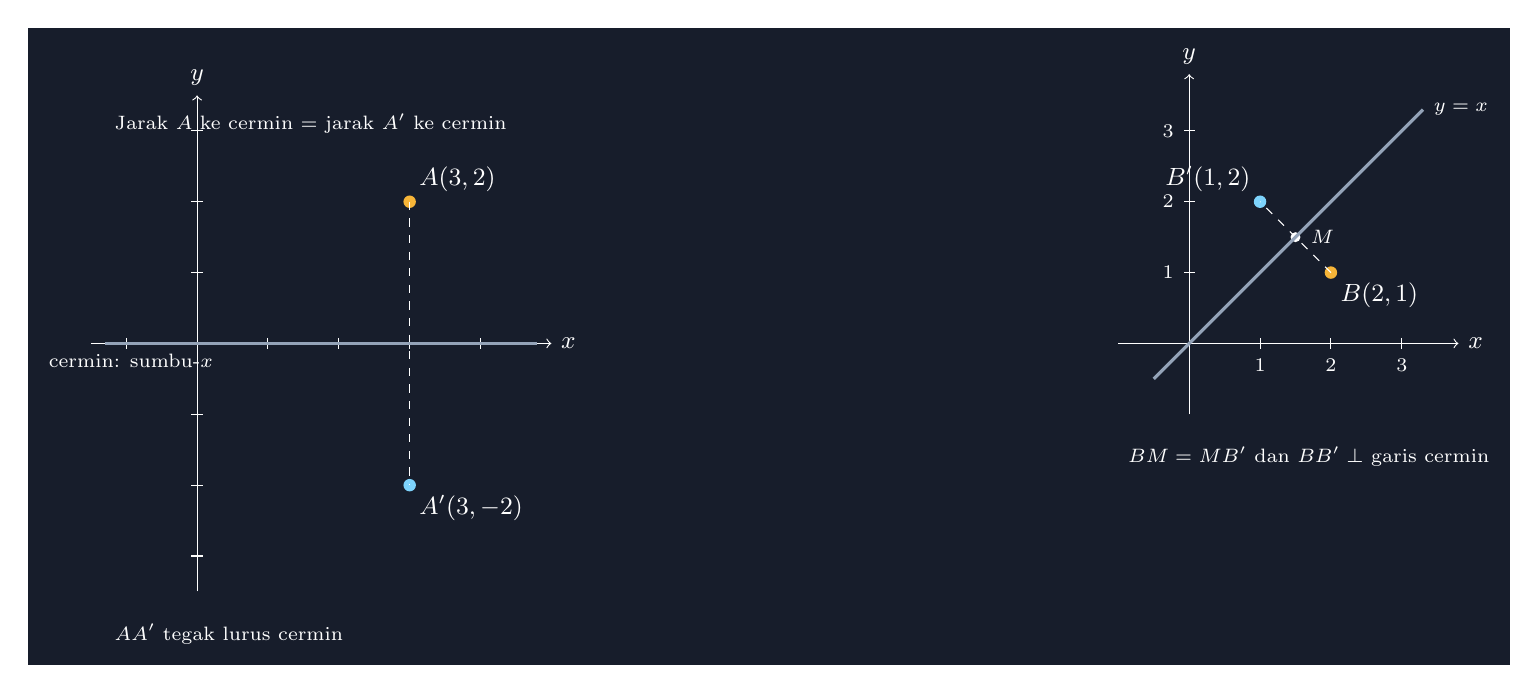
\begin{tikzpicture}[background rectangle/.style={fill=bg}, show background rectangle,
  every node/.style={text=putih, font=\small}]

  % ---------- Gambar 1: refleksi terhadap sumbu-x ----------
  \begin{scope}[scale=0.9, xshift=-1cm]
    \draw[->, putih!70] (-1.5,0) -- (5,0) node[right] {$x$};
    \draw[->, putih!70] (0,-3.5) -- (0,3.5) node[above] {$y$};
    \foreach \i in {-1,...,4}
      \draw[putih!40] (\i,0.08) -- (\i,-0.08);
    \foreach \j in {-3,...,3}
      \draw[putih!40] (0.08,\j) -- (-0.08,\j);

    \fill[aksen] (3,2) circle (2.5pt) node[above right] {$A(3,2)$};
    \fill[aksen2] (3,-2) circle (2.5pt) node[below right] {$A'(3,-2)$};
    \draw[dashed, putih!80] (3,2) -- (3,-2);
    \draw[very thick, cermin] (-1.3,0) -- (4.8,0)
      node[below, pos=0.06, font=\scriptsize] {cermin: sumbu-$x$};

    \node[putih!70, font=\scriptsize, anchor=west] at (-1.3,3.1)
      {Jarak $A$ ke cermin $=$ jarak $A'$ ke cermin};
    \node[putih!70, font=\scriptsize, anchor=west] at (-1.3,-4.1)
      {$AA'$ tegak lurus cermin};
  \end{scope}

  % ---------- Gambar 2: refleksi terhadap y = x ----------
  \begin{scope}[scale=0.9, xshift=13cm]
    \draw[->, putih!70] (-1,0) -- (3.8,0) node[right] {$x$};
    \draw[->, putih!70] (0,-1) -- (0,3.8) node[above] {$y$};
    \foreach \i in {1,2,3}
      \draw[putih!40] (\i,0.08) -- (\i,-0.08)
        node[below, font=\scriptsize, text=putih!70] {\i};
    \foreach \j in {1,2,3}
      \draw[putih!40] (0.08,\j) -- (-0.08,\j)
        node[left, font=\scriptsize, text=putih!70] {\j};

    \coordinate (B) at (2,1);
    \coordinate (M) at (1.5,1.5);
    \coordinate (Bp) at (1,2);

    \fill[aksen] (B) circle (2.5pt) node[below right] {$B(2,1)$};
    \fill[aksen2] (Bp) circle (2.5pt) node[above left] {$B'(1,2)$};
    \fill[putih] (M) circle (2pt) node[right=2pt, font=\scriptsize] {$M$};

    \draw[dashed, putih!80] (B) -- (Bp);
    \draw[very thick, cermin] (-0.5,-0.5) -- (3.3,3.3)
      node[right, font=\scriptsize] {$y=x$};

    \node[putih!70, font=\scriptsize, anchor=west] at (-1,-1.6)
      {$BM = MB'$ dan $BB' \perp$ garis cermin};
  \end{scope}

\end{tikzpicture}
\end{document}
